\documentclass[tikz, border=10pt]{standalone}
\usepackage{tikz}
\usepackage{amsmath}
\usetikzlibrary{arrows.meta}
\usetikzlibrary{positioning}
\usetikzlibrary{calc}

\begin{document}
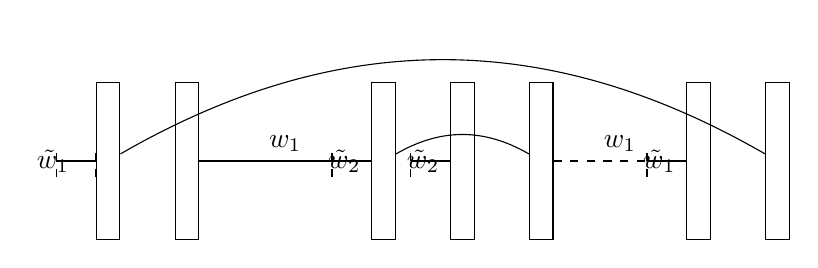
\begin{tikzpicture}[
    neuron/.style={rectangle, draw, minimum width=0.3cm, minimum height=2cm},
    neuron weight/.style={draw, line width=0.5pt, minimum width=0.5cm},
    connection/.style={draw, -},
    dashed connection/.style={draw, dashed}
]

% 第一组神经元(左侧)
\node[neuron] (n11) at (0,0) {};
\node[neuron] (n12) at (1,0) {};

% 第一组权重标记
\node (w11) at (-0.7,0) {$\tilde{w}_1$};
\draw (n11.west) -- ++(-0.5,0);
\draw (n11.west) ++(0,0) -- ++(0,0.1);
\draw (n11.west) ++(0,-0.1) -- ++(0,-0.1);
\draw (n11.west) ++(-0.5,0) -- ++(0,0.1);
\draw (n11.west) ++(-0.5,-0.1) -- ++(0,-0.1);

% 第二组神经元(中间)
\node[neuron] (n21) at (3.5,0) {};
\node[neuron] (n22) at (4.5,0) {};
\node[neuron] (n23) at (5.5,0) {};

% 第二组权重标记
\node (w21) at (3.0,0) {$\tilde{w}_2$};
\draw (n21.west) -- ++(-0.5,0);
\draw (n21.west) ++(0,0) -- ++(0,0.1);
\draw (n21.west) ++(0,-0.1) -- ++(0,-0.1);
\draw (n21.west) ++(-0.5,0) -- ++(0,0.1);
\draw (n21.west) ++(-0.5,-0.1) -- ++(0,-0.1);

\node (w22) at (4.0,0) {$\tilde{w}_2$};
\draw (n22.west) -- ++(-0.5,0);
\draw (n22.west) ++(0,0) -- ++(0,0.1);
\draw (n22.west) ++(0,-0.1) -- ++(0,-0.1);
\draw (n22.west) ++(-0.5,0) -- ++(0,0.1);
\draw (n22.west) ++(-0.5,-0.1) -- ++(0,-0.1);

% 第三组神经元(右侧)
\node[neuron] (n31) at (7.5,0) {};
\node[neuron] (n32) at (8.5,0) {};

% 第三组权重标记
\node (w31) at (7.0,0) {$\tilde{w}_1$};
\draw (n31.west) -- ++(-0.5,0);
\draw (n31.west) ++(0,0) -- ++(0,0.1);
\draw (n31.west) ++(0,-0.1) -- ++(0,-0.1);
\draw (n31.west) ++(-0.5,0) -- ++(0,0.1);
\draw (n31.west) ++(-0.5,-0.1) -- ++(0,-0.1);

% 连接线
\draw[connection] (n12) -- node[above, sloped] {$w_1$} (n21);
\draw[dashed connection] (n23) -- node[above, sloped] {$w_1$} (n31);

% 顶部弧线连接
\draw[connection] (n11) to[bend left=30] (n32);

% 中间弧线连接
\draw[connection] (n21) to[bend left=30] (n23);

\end{tikzpicture}
\end{document}